\section{Power Flow}

\begin{frame}{}
    \tableofcontents[currentsection]
\end{frame}

\begin{frame}{Power Flow Analysis}

Solving the Power Flow will allow as to find the steady-state powers and voltages of the system.\\
The PF equations will become the equality constraints of the optimization problem ($ \mathbf{H(x)} = 0$)
and its solution will determine the inequality contraints deviations and the active power losses:

\begin{equation}
    P_{losses} = (P_{owf} - P_{6}) \cdot S_{base} \cdot 10^{-6} \quad \text{MW}
\end{equation}

We will using the per-unit system:
\begin{equation}
    \text{Per unit value} = \frac{\text{Actual value}}{\text{Base value}}
\end{equation}
\begin{equation}
    \begin{cases}
        I_{base} = S_{base}V_{base} \\
        Y_{base} = \frac{S_{base}}{V_{base}^2} \\
    \end{cases}
\end{equation}
where $S_{base} =100 \text{ MVA}$ and $V_{base} = \text{ transmission voltage in kV}$.

\end{frame}


\subsection{Admittance Matrix and Equations}

\begin{frame}{Admittance matrix and equations}

Inspecting the Kirchhoff's Current Law (KCL) we can observe how the admittance matrix is the fundamental relationship between voltages and currents :
\begin{equation}
\textbf{I} = \textbf{Y}_{bus} \textbf{V}
\label{eq:kirchhoff}
\end{equation}

We have built $\textbf{Y}_{bus}$ by inspection applying KCL at each node. The expanded Power Flow equations become:
\begin{align}
    P_i= \sum_{k=1}^n|V_i||V_k|(G_{ik}cos(\theta_{ik}) + B_{ik}sin(\theta_{ik}))\label{powerflowP} \quad i= 1,2,...,n \\
    Q_i= \sum_{k=1}^n|V_i||V_k|(G_{ik}sin(\theta_{ik}) - B_{ik}cos(\theta_{ik}))\label{powerflowQ} \quad i= 1,2,...,n
\end{align}  
where $G_{ik}$ and $B_{ik}$ are the real and imaginary parts of $\textbf{Y}_{bus}$ respectively.
\end{frame}
    




\subsection{Newton-Raphson Method}

\begin{frame}{Newton-Raphson Method}

We will use the Newton-Raphson method is an iterative method to solve the set of Power Flow non-linear equations:

\begin{figure}
    \centering
    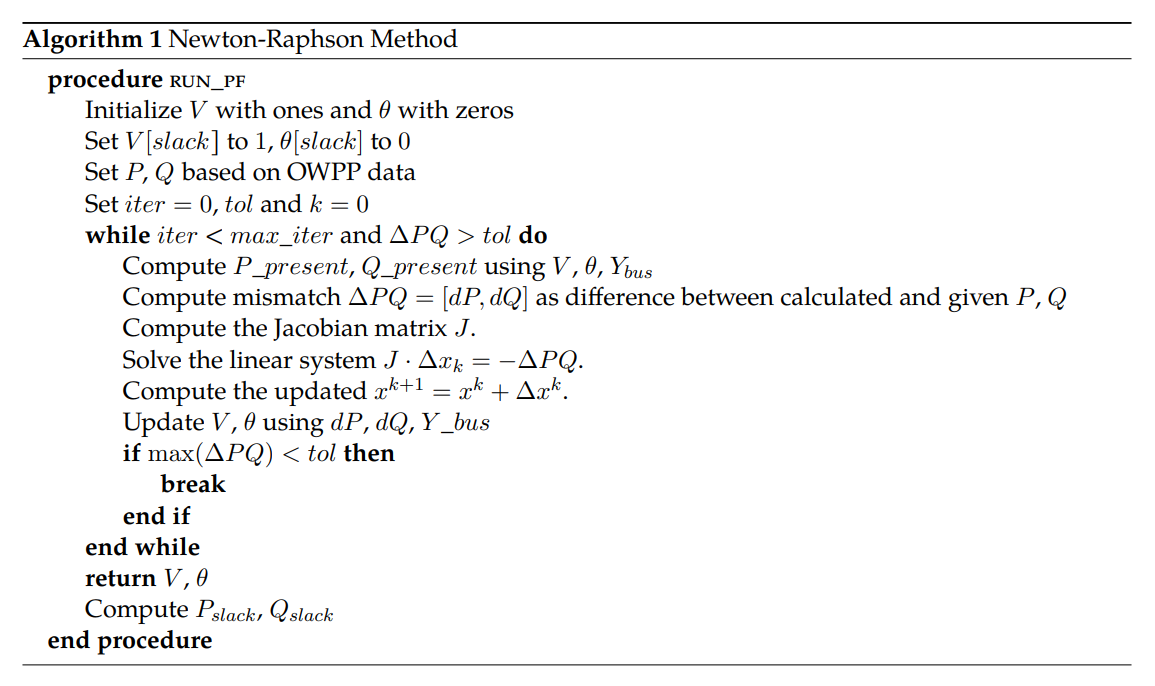
\includegraphics[width=0.8\textwidth]{imatges/NR_method.png}
    \caption{Newton-Raphson method.}
    \label{fig:newton_raphson}
\end{figure}
\end{frame}
